%% bare_conf.tex
%% V1.4
%% 2012/12/27
%% by Michael Shell
%% See:
%% http://www.michaelshell.org/
%% for current contact information.
%%
%% This is a skeleton file demonstrating the use of IEEEtran.cls
%% (requires IEEEtran.cls version 1.8 or later) with an IEEE conference paper.
%%
%% Support sites:
%% http://www.michaelshell.org/tex/ieeetran/
%% http://www.ctan.org/tex-archive/macros/latex/contrib/IEEEtran/
%% and
%% http://www.ieee.org/

%%*************************************************************************
%% Legal Notice:
%% This code is offered as-is without any warranty either expressed or
%% implied; without even the implied warranty of MERCHANTABILITY or
%% FITNESS FOR A PARTICULAR PURPOSE! 
%% User assumes all risk.
%% In no event shall IEEE or any contributor to this code be liable for
%% any damages or losses, including, but not limited to, incidental,
%% consequential, or any other damages, resulting from the use or misuse
%% of any information contained here.
%%
%% All comments are the opinions of their respective authors and are not
%% necessarily endorsed by the IEEE.
%%
%% This work is distributed under the LaTeX Project Public License (LPPL)
%% ( http://www.latex-project.org/ ) version 1.3, and may be freely used,
%% distributed and modified. A copy of the LPPL, version 1.3, is included
%% in the base LaTeX documentation of all distributions of LaTeX released
%% 2003/12/01 or later.
%% Retain all contribution notices and credits.
%% ** Modified files should be clearly indicated as such, including  **
%% ** renaming them and changing author support contact information. **
%%
%% File list of work: IEEEtran.cls, IEEEtran_HOWTO.pdf, bare_adv.tex,
%%                    bare_conf.tex, bare_jrnl.tex, bare_jrnl_compsoc.tex,
%%                    bare_jrnl_transmag.tex
%%*************************************************************************

% *** Authors should verify (and, if needed, correct) their LaTeX system  ***
% *** with the testflow diagnostic prior to trusting their LaTeX platform ***
% *** with production work. IEEE's font choices can trigger bugs that do  ***
% *** not appear when using other class files.                            ***
% The testflow support page is at:
% http://www.michaelshell.org/tex/testflow/



% Note that the a4paper option is mainly intended so that authors in
% countries using A4 can easily print to A4 and see how their papers will
% look in print - the typesetting of the document will not typically be
% affected with changes in paper size (but the bottom and side margins will).
% Use the testflow package mentioned above to verify correct handling of
% both paper sizes by the user's LaTeX system.
%
% Also note that the "draftcls" or "draftclsnofoot", not "draft", option
% should be used if it is desired that the figures are to be displayed in
% draft mode.
%
\documentclass[12pt,letter,final]{article}
% Add the compsoc option for Computer Society conferences.
%
% If IEEEtran.cls has not been installed into the LaTeX system files,
% manually specify the path to it like:
\usepackage[latin1]{inputenc}
\usepackage{amsfonts}
\usepackage{amssymb}
\usepackage{amsthm}
\usepackage{fullpage}
\usepackage{setspace}
\usepackage{graphicx}
%\usepackage[pdftex]{graphicx}
\usepackage{psfrag}
\usepackage{color}
\usepackage{epsfig}
\usepackage{appendix}
\usepackage{caption}
\usepackage{cite}
\usepackage{ifpdf}
\usepackage[cmex10]{amsmath}
\usepackage{algorithmic}
\usepackage{array}
\usepackage{stfloats}
\usepackage{url}
\usepackage{fixltx2e}
\usepackage{setspace} 
\usepackage{diagbox}
\usepackage{subfigure}





% Some very useful LaTeX packages include:
% (uncomment the ones you want to load)


% *** MISC UTILITY PACKAGES ***
%
%\usepackage{ifpdf}
% Heiko Oberdiek's ifpdf.sty is very useful if you need conditional
% compilation based on whether the output is pdf or dvi.
% usage:
% \ifpdf
%   % pdf code
% \else
%   % dvi code
% \fi
% The latest version of ifpdf.sty can be obtained from:
% http://www.ctan.org/tex-archive/macros/latex/contrib/oberdiek/
% Also, note that IEEEtran.cls V1.7 and later provides a builtin
% \ifCLASSINFOpdf conditional that works the same way.
% When switching from latex to pdflatex and vice-versa, the compiler may
% have to be run twice to clear warning/error messages.






% *** CITATION PACKAGES ***
%
%\usepackage{cite}
% cite.sty was written by Donald Arseneau
% V1.6 and later of IEEEtran pre-defines the format of the cite.sty package
% \cite{} output to follow that of IEEE. Loading the cite package will
% result in citation numbers being automatically sorted and properly
% "compressed/ranged". e.g., [1], [9], [2], [7], [5], [6] without using
% cite.sty will become [1], [2], [5]--[7], [9] using cite.sty. cite.sty's
% \cite will automatically add leading space, if needed. Use cite.sty's
% noadjust option (cite.sty V3.8 and later) if you want to turn this off
% such as if a citation ever needs to be enclosed in parenthesis.
% cite.sty is already installed on most LaTeX systems. Be sure and use
% version 4.0 (2003-05-27) and later if using hyperref.sty. cite.sty does
% not currently provide for hyperlinked citations.
% The latest version can be obtained at:
% http://www.ctan.org/tex-archive/macros/latex/contrib/cite/
% The documentation is contained in the cite.sty file itself.






% *** GRAPHICS RELATED PACKAGES ***
%
%\ifCLASSINFOpdf
  % \usepackage[pdftex]{graphicx}
  % declare the path(s) where your graphic files are
  % \graphicspath{{../pdf/}{../jpeg/}}
  % and their extensions so you won't have to specify these with
  % every instance of \includegraphics
  % \DeclareGraphicsExtensions{.pdf,.jpeg,.png}
%\else
  % or other class option (dvipsone, dvipdf, if not using dvips). graphicx
  % will default to the driver specified in the system graphics.cfg if no
  % driver is specified.
  % \usepackage[dvips]{graphicx}
  % declare the path(s) where your graphic files are
  % \graphicspath{{../eps/}}
  % and their extensions so you won't have to specify these with
  % every instance of \includegraphics
  % \DeclareGraphicsExtensions{.eps}
%\fi
% graphicx was written by David Carlisle and Sebastian Rahtz. It is
% required if you want graphics, photos, etc. graphicx.sty is already
% installed on most LaTeX systems. The latest version and documentation
% can be obtained at: 
% http://www.ctan.org/tex-archive/macros/latex/required/graphics/
% Another good source of documentation is "Using Imported Graphics in
% LaTeX2e" by Keith Reckdahl which can be found at:
% http://www.ctan.org/tex-archive/info/epslatex/
%
% latex, and pdflatex in dvi mode, support graphics in encapsulated
% postscript (.eps) format. pdflatex in pdf mode supports graphics
% in .pdf, .jpeg, .png and .mps (metapost) formats. Users should ensure
% that all non-photo figures use a vector format (.eps, .pdf, .mps) and
% not a bitmapped formats (.jpeg, .png). IEEE frowns on bitmapped formats
% which can result in "jaggedy"/blurry rendering of lines and letters as
% well as large increases in file sizes.
%
% You can find documentation about the pdfTeX application at:
% http://www.tug.org/applications/pdftex





% *** MATH PACKAGES ***
%
%\usepackage[cmex10]{amsmath}
% A popular package from the American Mathematical Society that provides
% many useful and powerful commands for dealing with mathematics. If using
% it, be sure to load this package with the cmex10 option to ensure that
% only type 1 fonts will utilized at all point sizes. Without this option,
% it is possible that some math symbols, particularly those within
% footnotes, will be rendered in bitmap form which will result in a
% document that can not be IEEE Xplore compliant!
%
% Also, note that the amsmath package sets \interdisplaylinepenalty to 10000
% thus preventing page breaks from occurring within multiline equations. Use:
%\interdisplaylinepenalty=2500
% after loading amsmath to restore such page breaks as IEEEtran.cls normally
% does. amsmath.sty is already installed on most LaTeX systems. The latest
% version and documentation can be obtained at:
% http://www.ctan.org/tex-archive/macros/latex/required/amslatex/math/





% *** SPECIALIZED LIST PACKAGES ***
%
%\usepackage{algorithmic}
% algorithmic.sty was written by Peter Williams and Rogerio Brito.
% This package provides an algorithmic environment fo describing algorithms.
% You can use the algorithmic environment in-text or within a figure
% environment to provide for a floating algorithm. Do NOT use the algorithm
% floating environment provided by algorithm.sty (by the same authors) or
% algorithm2e.sty (by Christophe Fiorio) as IEEE does not use dedicated
% algorithm float types and packages that provide these will not provide
% correct IEEE style captions. The latest version and documentation of
% algorithmic.sty can be obtained at:
% http://www.ctan.org/tex-archive/macros/latex/contrib/algorithms/
% There is also a support site at:
% http://algorithms.berlios.de/index.html
% Also of interest may be the (relatively newer and more customizable)
% algorithmicx.sty package by Szasz Janos:
% http://www.ctan.org/tex-archive/macros/latex/contrib/algorithmicx/




% *** ALIGNMENT PACKAGES ***
%
%\usepackage{array}
% Frank Mittelbach's and David Carlisle's array.sty patches and improves
% the standard LaTeX2e array and tabular environments to provide better
% appearance and additional user controls. As the default LaTeX2e table
% generation code is lacking to the point of almost being broken with
% respect to the quality of the end results, all users are strongly
% advised to use an enhanced (at the very least that provided by array.sty)
% set of table tools. array.sty is already installed on most systems. The
% latest version and documentation can be obtained at:
% http://www.ctan.org/tex-archive/macros/latex/required/tools/


% IEEEtran contains the IEEEeqnarray family of commands that can be used to
% generate multiline equations as well as matrices, tables, etc., of high
% quality.




% *** SUBFIGURE PACKAGES ***
%\ifCLASSOPTIONcompsoc
%  \usepackage[caption=false,font=normalsize,labelfont=sf,textfont=sf]{subfig}
%\else
%  \usepackage[caption=false,font=footnotesize]{subfig}
%\fi
% subfig.sty, written by Steven Douglas Cochran, is the modern replacement
% for subfigure.sty, the latter of which is no longer maintained and is
% incompatible with some LaTeX packages including fixltx2e. However,
% subfig.sty requires and automatically loads Axel Sommerfeldt's caption.sty
% which will override IEEEtran.cls' handling of captions and this will result
% in non-IEEE style figure/table captions. To prevent this problem, be sure
% and invoke subfig.sty's "caption=false" package option (available since
% subfig.sty version 1.3, 2005/06/28) as this is will preserve IEEEtran.cls
% handling of captions.
% Note that the Computer Society format requires a larger sans serif font
% than the serif footnote size font used in traditional IEEE formatting
% and thus the need to invoke different subfig.sty package options depending
% on whether compsoc mode has been enabled.
%
% The latest version and documentation of subfig.sty can be obtained at:
% http://www.ctan.org/tex-archive/macros/latex/contrib/subfig/




% *** FLOAT PACKAGES ***
%
%\usepackage{fixltx2e}
% fixltx2e, the successor to the earlier fix2col.sty, was written by
% Frank Mittelbach and David Carlisle. This package corrects a few problems
% in the LaTeX2e kernel, the most notable of which is that in current
% LaTeX2e releases, the ordering of single and double column floats is not
% guaranteed to be preserved. Thus, an unpatched LaTeX2e can allow a
% single column figure to be placed prior to an earlier double column
% figure. The latest version and documentation can be found at:
% http://www.ctan.org/tex-archive/macros/latex/base/


%\usepackage{stfloats}
% stfloats.sty was written by Sigitas Tolusis. This package gives LaTeX2e
% the ability to do double column floats at the bottom of the page as well
% as the top. (e.g., "\begin{figure*}[!b]" is not normally possible in
% LaTeX2e). It also provides a command:
%\fnbelowfloat
% to enable the placement of footnotes below bottom floats (the standard
% LaTeX2e kernel puts them above bottom floats). This is an invasive package
% which rewrites many portions of the LaTeX2e float routines. It may not work
% with other packages that modify the LaTeX2e float routines. The latest
% version and documentation can be obtained at:
% http://www.ctan.org/tex-archive/macros/latex/contrib/sttools/
% Do not use the stfloats baselinefloat ability as IEEE does not allow
% \baselineskip to stretch. Authors submitting work to the IEEE should note
% that IEEE rarely uses double column equations and that authors should try
% to avoid such use. Do not be tempted to use the cuted.sty or midfloat.sty
% packages (also by Sigitas Tolusis) as IEEE does not format its papers in
% such ways.
% Do not attempt to use stfloats with fixltx2e as they are incompatible.
% Instead, use Morten Hogholm'a dblfloatfix which combines the features
% of both fixltx2e and stfloats:
%
% \usepackage{dblfloatfix}
% The latest version can be found at:
% http://www.ctan.org/tex-archive/macros/latex/contrib/dblfloatfix/




% *** PDF, URL AND HYPERLINK PACKAGES ***
%
%\usepackage{url}
% url.sty was written by Donald Arseneau. It provides better support for
% handling and breaking URLs. url.sty is already installed on most LaTeX
% systems. The latest version and documentation can be obtained at:
% http://www.ctan.org/tex-archive/macros/latex/contrib/url/
% Basically, \url{my_url_here}.




% *** Do not adjust lengths that control margins, column widths, etc. ***
% *** Do not use packages that alter fonts (such as pslatex).         ***
% There should be no need to do such things with IEEEtran.cls V1.6 and later.
% (Unless specifically asked to do so by the journal or conference you plan
% to submit to, of course. )


% correct bad hyphenation here
%\hyphenation{op-tical net-works semi-conduc-tor}



%
% paper title
% can use linebreaks \\ within to get better formatting as desired
% Do not put math or special symbols in the title.
\title{Report}


% author names and affiliations
% use a multiple column layout for up to three different
% affiliations
%\author{\IEEEauthorblockN{Tianpei Chen}
%\IEEEauthorblockA{ID: 25504946\\Department of Electrical and\\Computer Engineering\\
%McGill University\\
%Montreal, Quebec}}
\author{Tianpei Chen\\
 Department of Electrical and Computer Engineering\\
 McGill University}

% conference papers do not typically use \thanks and this command
% is locked out in conference mode. If really needed, such as for
% the acknowledgment of grants, issue a \IEEEoverridecommandlockouts
% after \documentclass

% for over three affiliations, or if they all won't fit within the width
% of the page, use this alternative format:
% 
%\author{\IEEEauthorblockN{Michael Shell\IEEEauthorrefmark{1},
%Homer Simpson\IEEEauthorrefmark{2},
%James Kirk\IEEEauthorrefmark{3}, 
%Montgomery Scott\IEEEauthorrefmark{3} and
%Eldon Tyrell\IEEEauthorrefmark{4}}
%\IEEEauthorblockA{\IEEEauthorrefmark{1}School of Electrical and Computer Engineering\\
%Georgia Institute of Technology,
%Atlanta, Georgia 30332--0250\\ Email: see http://www.michaelshell.org/contact.html}
%\IEEEauthorblockA{\IEEEauthorrefmark{2}Twentieth Century Fox, Springfield, USA\\
%Email: homer@thesimpsons.com}
%\IEEEauthorblockA{\IEEEauthorrefmark{3}Starfleet Academy, San Francisco, California 96678-2391\\
%Telephone: (800) 555--1212, Fax: (888) 555--1212}
%\IEEEauthorblockA{\IEEEauthorrefmark{4}Tyrell Inc., 123 Replicant Street, Los Angeles, California 90210--4321}}




% use for special paper notices
%\IEEEspecialpapernotice{(Invited Paper)}
\begin{document}
% make the title area
\begin{spacing}{2.5}
\maketitle
\section{Introduction}
Detection algorithm is one of the key components of Multiple-Input Multiple-Output (MIMO) systems. Designing of high performance and low complexity detector has become a bottleneck of Large MIMO systems. Recently, academia has found a property of large MIMO channel called channel hardening phenomenon \cite{hochwald2004multiple}\cite{tse2005fundamentals}\cite{marvcenko1967distribution}\cite{tulino2004random}, which states the phenomenon that with the number of receiving or transmitting antennas increasing, the variances of channel mutual information decrease. Simply saying, the channel "hardens". An useful aspect of channel hardening phenomenon is the off diagonal elements of $\mathbf{H}^{H}\mathbf{H}$ matrix becomes more and more ignorable comparing to diagonal elements when the number of receiving antennas or transmitting antennas becomes large.

 Channel hardening phenomenon provides an opportunity for designing computationally economical detection algorithms. For example, linear detectors (LDs) such as zero forcing (ZF) and minimum mean square error (MMSE) detectors need to calculate the inverse of $\mathbf{H}^{H}\mathbf{H}$ matrix. This process can be accelerated by approximate matrix inversion using series expansion techniques and deterministic approximations in large dimensions\cite{wu2013approximate}. Channel hardening phenomenon can also provide computational advances to machine learning based detectors, e.g. probability data association (PDA)\cite{fricke1900impact}\cite{pham2004generalized} and message passing detectors\cite{som2011low}\cite{goldberger2011mimo}\cite{lakshmi2013channel} and Monte-Carlo Markov Chain (MCMC) MIMO detectors\cite{farhang2006markov}\cite{datta2012novel}. This type of algorithms work well in large sparse systems.
 
In this report, we propose some useful insights of the orthogonal properties of channel. We define orthogonality measurement (om), which is a well round metric that considers both diagonal and off diagonal elements of $\mathbf{H}^{H}\mathbf{H}$.

The rest of the report is organized as follows, section \ref{system model} introduces system model. Section \ref{preliminary} provides some preliminaries of the definition of orthogonality measurement. Section \ref{log expectation of om} discusses the derivation of logarithmic expectation of orthogonality measurement. In section \ref{pdf of om} we obtain probability density function of orthogonality measurement. Some computer simulation results are presented in section \ref{computer simulation}.


\section{System Model}\label{system model}
We consider a complex uncoded spatial multiplexing MIMO system with $N_r$ receive and $N_t$ transmit antennas, $N_{r}\geq N_{t}$, over a flat fading channel. Using a discrete time model, $\mathbf{y}\in\mathbb{C}^{N_{r}\times 1}$ is the received symbol vector written as:
\begin{equation}
\mathbf{y}=\mathbf{H}\mathbf{s}+\mathbf{n},   \label{formula 1}
\end{equation}
where $\mathbf{s}\in \mathbb{C}^{N_{t}\times 1}$ is the transmitted symbol vector, with components that are mutually independent and taken from a finite signal constellation alphabet $\mathbb{O}$ (e.g. 4-QAM, 16-QAM, 64-QAM) of size $M$. The possible transmitted symbol vectors $\mathbf{s}\in \mathbb{O}^{N_{t}}$, satisfy $\mathbb{E}[\mathbf{s}\mathbf{s}^{H}]=\mathbf{I}_{N_t}E_{s}$, where $E_{s}$ denotes the symbol average energy, and $\mathbb{E}[\cdot]$ denotes the expectation operation. Furthermore $\mathbf{H}\in \mathbb{C}^{N_{r}\times N_{t}}$ denotes the Rayleigh fading channel propagation matrix with independent identically distributed (i.i.d) circularly symmetric complex Gaussian components of zero mean and unit variance. Finally, $\mathbf{n}\in \mathbb{C}^{N_{r}\times 1}$ is the additive white Gaussian noise (AWGN) vector with zero mean components and $\mathbb{E}[\mathbf{n}\mathbf{n}^{H}]=\mathbf{I}_{N_{r}}N_{0}$, where $N_{0}$ denotes the noise power spectrum density, and hence $\frac{E_{s}}{N_{0}}$ is the signal to noise ratio (SNR). 

Assume the receiver has perfect channel state information (CSI), meaning that $ \mathbf{H}$ is known, as well as the SNR. The task of the MIMO decoder is to recover $\mathbf{s}$ based on $\mathbf{y}$ and $\mathbf{H}$.
\section{Preliminaries}\label{preliminary}
Orthogonality deficiency measures the how orthogonal a matrix is \cite{ma2008performance}, which is defined by
\begin{equation}
\phi_{od}=1-\frac{det(\mathbf{W})}{\prod_{i=1}^{N_{t}}||\mathbf{h}_{i}||^{2}},
\label{formula1}
\end{equation}
where $\mathbf{W}=\mathbf{H}^{H}\mathbf{H}$ denotes Wishart matrix, $\mathbf{h}_{i}$ denotes the $i$ th column of $\mathbf{H}$, $det(\cdot)$ denotes determinant operation, $||\cdot||^{2}$ denotes 2-norm operation.
In (\ref{formula1}), $||\mathbf{h}_{i}||^{2}=\sum_{i=1}^{N_{t}}|\mathbf{H}_{ij}|^{2}$, $\mathbf{H}_{ij}$ denotes the component of $\mathbf{H}$ at $i$ th row and $j$ th column. $\mathbf{H}_{ij}\sim Rayleigh(1/\sqrt{2})$, therefore $||\mathbf{h}_{i}||^{2}\sim Gamma(N_{r},1)$\cite{papoulis1996stochastic}. $Gamma(k,\theta)$ denotes Gamma distribution, with $k$ degrees of freedom. Furthermore, we have:
\begin{equation}
2||\mathbf{h}_{i}||^{2}\sim Gamma(N_{r},2)\sim\chi^{2}_{2N_{r}},
\label{formula2}
\end{equation} 
$\chi^{2}_{k}$ denotes chi-square distribution with $k$ degrees of freedom. For the sake of simplicity, (\ref{formula1}) can be changed to:
\begin{equation}
\phi_{om}=\frac{det(\mathbf{W})}{\prod_{i=1}^{N_{t}}||\mathbf{h}_{i}||^{2}}=\frac{2^{N_{t}}det(\mathbf{W})}{\prod_{i=1}^{N_{t}}2||\mathbf{h}_{i}||^{2}}.
\label{formula3}
\end{equation}
Taking logarithmic operation to $\phi_{om}$ we have 
\begin{equation}
\ln(\phi_{om})=N_{t}\ln(2)+\ln(det(\mathbf{W}))-\sum_{i=1}^{N_{t}}\ln(2||\mathbf{h}_{i}||^{2}),
\label{formula4}
\end{equation}
$\phi_{om}$ in (\ref{formula3}) is defined as Orthogonality Measure. Based on Hadamard's inequality ($\prod_{i=1}^{N_{t}}||\mathbf{h}_{i}||\geq det(\mathbf{H})$). $\phi_{om}\in [0,1]$. If $\phi_{om}$ is more closer to 1, $\mathbf{H}$ is closer to orthogonal matrix.

Because $\mathbf{W}=\mathbf{H}^{H}\mathbf{H}$, do QR factorization to $\mathbf{H}$ 
\begin{equation}
\mathbf{H}=\mathbf{Q}\mathbf{R},
\label{formula5} 
 \end{equation}
where $\mathbf{Q}\in\mathbb{C}^{N_{r}\times N_{t}}$ is a unitary matrix and $\mathbf{R}\in\mathbb{C}^{N_{t}\times N_{t}}$ is the upper triangular matrix. Using (\ref{formula5}), we have $\mathbf{W}=\mathbf{R}^{H}\mathbf{R}$. $r_{ii}$ denotes the $i$ th diagonal component of $\mathbf{R}$, thus $det(\mathbf{W})$ can be rewritten as:
\begin{equation}
det(\mathbf{W})=det(\mathbf{R}^{H}\mathbf{R})=det(\mathbf{R}^{H})det(\mathbf{R})\\=\prod_{i=1}^{N_{t}}r_{ii}^{H}\prod_{i=1}^{N_{t}}r_{ii}=\prod_{i=1}^{N_{t}}|r_{ii}|^{2}.
\label{formula6}
\end{equation}  
Notice that $\mathbf{R}$ can be viewed as the Cholesky factorization of $\mathbf{W}$. Therefore, we have
\begin{equation}
 ||\mathbf{h}_{i}||^{2}=\mathbf{W}_{ii}=\sum^{i-1}_{j=1}|r_{ji}|^{2}+|r_{ii}|^{2},
\label{formula7}
 \end{equation}
 where $\mathbf{W}_{ii}$ denotes the $i$ th diagonal element of $\mathbf{W}$.
 Thus based on (\ref{formula6}) and (\ref{formula7}), (\ref{formula3}) can be rewritten as:
\begin{equation}
\phi_{om}=\prod_{i=1}^{N_{t}}\frac{|r_{ii}|^{2}}{|r_{ii}|^{2}+\sum^{i-1}_{j=1}|r_{ji}|^{2}}.
\label{formula9}
\end{equation}  
\section{Logarithmic Expectation of Orthogonality Measurement}\label{log expectation of om}

Taking expectation of (\ref{formula4}), we have 
\begin{equation}
\mathbb{E}[\ln(\phi_{om})]=N_{t}\ln(2)+\mathbb{E}[\ln(det(\mathbf{W}))]-\sum_{i=1}^{N_{t}}\mathbb{E}[\ln(2||\mathbf{h}_{i}||^{2})].
\label{formula11}
\end{equation}
Consider $\mathbf{H}=[\mathbf{h}_{1}^{'},\mathbf{h}_{2}^{'},\cdots \mathbf{h}_{N_{r}}^{'}]^{'}$, where $\mathbf{h}_{i}$ denotes the $i$ th row of $\mathbf{H}$, because each component of $\mathbf{H}$ is mutually independent and subject to circularly symmetric complex Gaussian distribution, i.e. $h_{i}\sim \mathbb{C}N(\mathbf{0},\mathbf{I}_{N_{t}})$. Therefore, $\mathbf{W}=\mathbf{H}^{H}\mathbf{H}\sim \mathbb{C}W(N_{r}, \mathbf{I}_{N_{t}})$, $\mathbb{C}W(n,\mathbf{\Sigma})$ denotes complex Wishart distribution with $n$ degrees of freedom and covariance matrix $\mathbf{\Sigma}$. The logarithmic expectation of $\mathbf{W}$ can be rewritten as
\begin{equation}
\mathbb{E}[\ln(det(\mathbf{W}))]=\frac{\tilde{\Gamma}^{'}_{N_{t}}(N_{r})}{\tilde{\Gamma}_{N_{t}}(N_{r})}=\sum_{i=1}^{N_{t}}\psi(N_{r}-i+1),
\label{formula12}
\end{equation}
where $\tilde{\Gamma}_{m}(n)$ denotes the multivariate Gamma function. Proof: see Appendix A.

Because the logarithmic expectation of a Gamma distribution variable $\mathbb{g}\sim Gamma(n,\theta)$ can be written as:
\begin{equation}
\mathbb{E}[\ln(\mathbb{g})]=\psi(n)+\ln(\theta),
\end{equation}
where $\psi(n)$ denotes Digamma function. Thus according to (\ref{formula2}), we have:
\begin{equation}
\mathbb{E}[\ln(2||\mathbf{h}_{i}||^{2})]=\psi(N_{r})+\ln(2).
\label{formula14}
\end{equation}
Proof: see Appendix B
Based on (\ref{formula11})(\ref{formula12})(\ref{formula14}), The logarithmic expectation of $\phi_{om}$ can be written as:
\begin{eqnarray}
\nonumber
\mathbb{E}[\ln(\phi_{om})]&=&N_{t}\ln(2)+\sum_{i=1}^{N_{t}}\psi(N_{r}-i+1)-N_{t}\psi(N_{r})-N_{t}\ln(2)\\
&=& \sum_{i=1}^{N_{t}}\psi(N_{r}-i+1)-N_{t}\psi(N_{r})
\label{formula15}
\end{eqnarray}
\section{Probability Density Function of Orthogonality Measurement}\label{pdf of om}
Recall (\ref{formula9})
\begin{equation}
\phi_{om}=\prod_{i=1}^{N_{t}}\frac{|r_{ii}|^{2}}{|r_{ii}|^{2}+\sum_{j<i}|r_{ji}|^{2}}.
\end{equation}
All the components in $\mathbf{R}$ are independently distributed and $r_{ji}\sim \mathbb{C}N(0,1)$, $|r_{ii}|^{2}\sim Gamma((N_{r}-i+1),1)$ \cite{nagar2011expectations}. Because $|r_{ji}|\sim Rayleigh(1/\sqrt{2})$, $\sum_{j<i}|r_{ji}|^{2}\sim Gamma(i-1, 1)$. Defining $\alpha_{i}=\sum_{j<i}|r_{ji}|^{2}$ and $\beta_{i}=|r_{ii}|^{2}$, $\alpha_{i}$ and $\beta_{i}$ are mutually independent, therefore (\ref{formula9}) can be rewritten to 
\begin{equation}
\phi_{om}=\prod_{i=1}^{N_{t}}\frac{\beta_{i}}{\alpha_{i}+\beta_{i}},
\label{formula21}
\end{equation}
From \cite{gupta2004handbook}, if $X\sim Gamma(k_{1},\theta)$ and $Y\sim Gamma(k_{2},\theta)$, then $\frac{X}{X+Y}\sim B(k_{1},k_{2})$, where $B$ denotes Beta distribution. Therefore $\frac{\beta_{i}}{\beta_{i}+\alpha_{i}}\sim B(k^{i}_{1}, k^{i}_{2})$, where $k^{i}_{1}=N_{r}-i+1$, $k^{i}_{2}=i-1$. we define $\eta_{i}=\frac{\beta_{i}}{\beta_{i}+\alpha_{i}}$, it is obvious that $\eta_{i}$ are independently distributed. Based on (\ref{formula21}), we have 
\begin{equation}
\phi_{om}=\prod_{i=1}^{N_{t}}\eta_{i}.
\label{formula22}
\end{equation}
Therefore the density function of $\phi_{om}$ can be defined as
\begin{equation}
f_{\phi_{om}}(x)=\frac{1}{x}\sum_{\mathbf{j}}(\prod_{i=1}^{N_{t}}c(k_{1}^{i}k,k_{2}^{i},j^{i}))f(\ln(x)|\mathbf{k_{1}}+\mathbf{j}), 
\label{formula23}
\end{equation}
where $\sum_{\mathbf{j}}=\sum_{j^{1}}\sum_{j^{2}}\cdots \sum_{j^{N_{t}}}$, the range of $j^{i}\in [0, k_{2}^{i}-1]$, $c(k_{1}^{i}, k_{2}^{i}, j_{i})=(-1)^{j^{i}}$ $k_{2}^{i}-1\choose j^{i}$ $[(k_{1}^{i}+k_{2}^{i})\mathbb{B}(k_{1}^{i},k_{2}^{i})]^{-1}$, $\mathbb{B}(\alpha, \beta)$ denotes beta function. $f(\ln(x)|\mathbf{k_{1}}+\mathbf{j})=(\prod_{i=1}^{N_{t}}(k_{1}^{i}+j^{i}))\sum_{i=1}^{N_{t}}[exp((k_{1}^{i}+j^{i})\ln(x))/\prod_{j=1\\ j\neq i}^{N_{t}}(k_{1}^{j}+j^{j}-k_{1}^{i}-j^{i})]$. $\mathbf{k_{1}}+\mathbf{j}=[k_{1}^{1}+j^{1},\cdots k_{1}^{N_{t}-1}+j^{N_{t}-1},k_{1}^{N_{t}}+j^{N_{t}}]$. Proof: see Appendix C. 

Consider logarithmic expectation of $\phi_{om}$, we have
\begin{equation}
E[\ln(\phi_{om})]=\sum_{i=1}^{N_{t}}E[\ln(\eta_{i})],
\label{formula24}
\end{equation}
where $E[\ln(\eta_{i})]=\psi(k^{i}_{1})-\psi(k^{i}_{1}+k^{i}_{2})$, thus we have 
\begin{equation}
E[\ln(\phi_{om})]=\sum_{i=1}^{N_{t}}\psi(N_{r}-i+1)-N_{t}\psi(N_{r}).
\label{formula25}
\end{equation}
we can find (\ref{formula25}) is consistent with (\ref{formula15}). 

\section{Computer Simulations}\label{computer simulation}
 Computer simulations are made for different sizes of V-BLAST MIMO systems, with $5\leq N_{r} \leq 100, 5 \leq N_{t} \leq N_{r}$, the empirical estimation of logarithmic expectation of $\phi_{om}$, $E[\ln(\phi_{om})]_{em}$, is calculated by taking average over $1e4$ channel realizations for each size of MIMO systems, as shown in Fig. \ref{figure1}, the Theoretical logarithmic expectation of $\phi_{om}$ $E[\ln(\phi_{om})]_{t}$ in (\ref{formula25}) is plotted in Fig. \ref{figure2}. Average deviation between $E[\ln(\phi_{om})]_{em}$ and $E[\ln(\phi_{om})]_{t}$ is also calculated, $V_{em-t}= 7.3043e-04$.




\begin{figure}[htb]
\centering
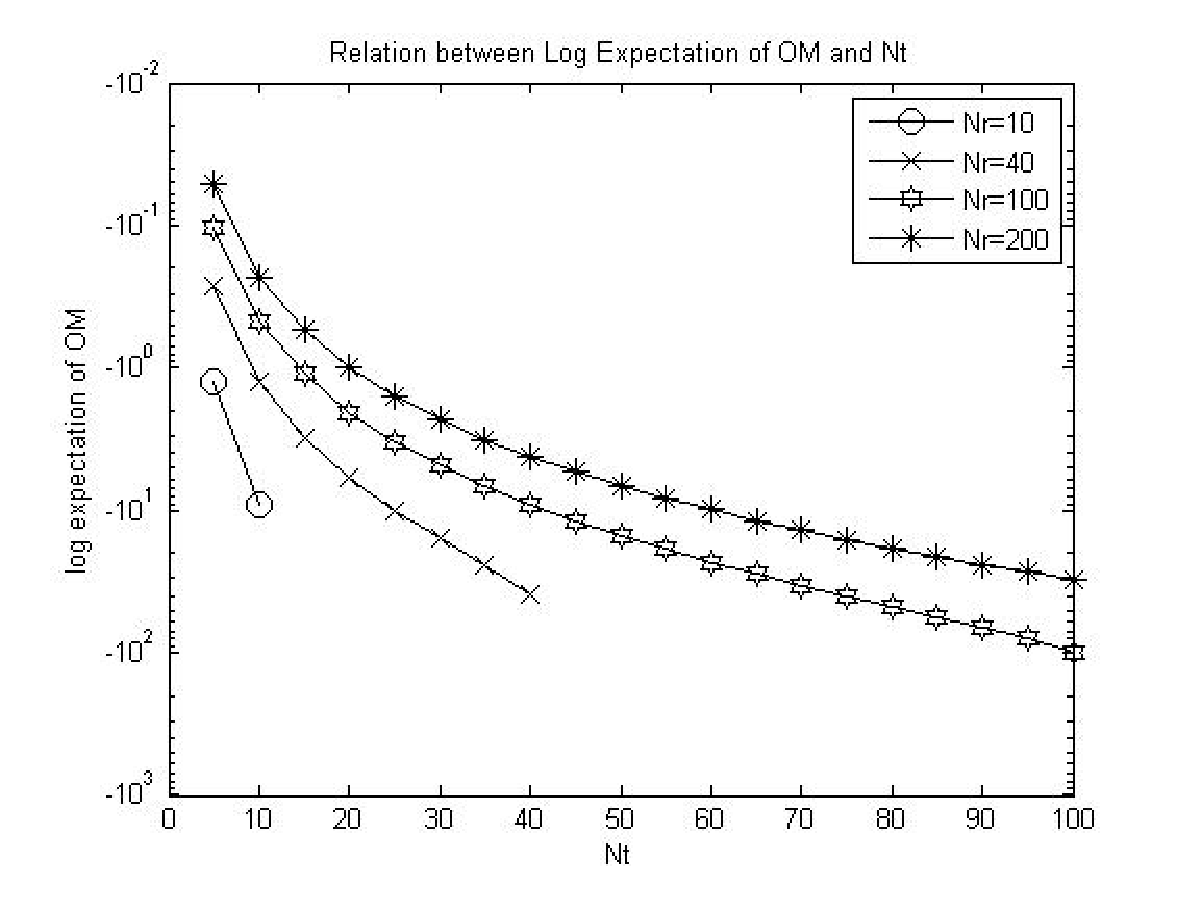
\includegraphics[scale=0.6]{NtE.eps}
\caption{Relation between $N_{t}$ and $E[\ln(\phi_{om})]_{t}$}
\label{figure3}
\end{figure}

Fig. \ref{figure3} demonstrates the relation between the number of users ($N_{t}$) and $E[\ln(\phi_{om})]_{t}$ under cases of different numbers of antennas at base station ($N_{r}$). From Fig. \ref{figure3}, we can see, on the one hand, with $N_{r}$ fixed, $E[\ln(\phi_{om})]$ decreases while $N_{t}$ increases, however the gradient of each curve becomes more and more gentle. On the other hand, when $N_{r}$ becomes larger $E[\ln(\phi_{om})]$ becomes more insensitive to variation of $N_{t}$.
\begin{figure}[htb]
\centering
\centering\includegraphics[width=0.7\textwidth, height=5cm]{LogE_om_em.eps}
\caption{Empirical Estimation $E[\ln(\phi_{om})]_{em}$}
\label{figure1}
\end{figure}

\begin{figure}[htb]
\centering
\includegraphics[width=0.7\textwidth, height=5cm]{LogE_om_t.eps}
\caption{Theoretical $E[\ln(\phi_{om})]_{t}$}
\label{figure2}
\end{figure} 

\begin{appendices}
\section{Appendix A}
Let $\mathbf{A}\in \mathbb{C}^{m\times m}$, $A\sim \mathbb{C}W(n, \mathbf{\Sigma})$, $\mathbb{C}W(n, \mathbf{\Sigma})$ denotes complex Wishart distribution with $n$ degrees of freedom and covariance matrix $\mathbf{\Sigma}$. It is obvious $\mathbf{A}$ is Hermition positive definite matrix, $\mathbf{A}=\mathbf{A}^{H}>0$.

The p.d.f function of $\mathbf{A}$ can be written as\cite{nagar2011expectations}:
\begin{equation}
f(A)=\{\tilde{\Gamma}_{m}(n)det(\mathbf{\Sigma})^{n} \}^{-1}det(A)^{n-m}etr(-\mathbf{\Sigma}^{-1}\mathbf{A}),
\label{Appendequa1}
\end{equation}
where $\tilde{\Gamma}_{m}(\beta)$ denotes multivariate complex Gamma function defined by:
\begin{equation}
\tilde{\Gamma}_{m}(\beta)=\pi^{\frac{m(m-1)}{2}}\prod_{i=1}^{m}\Gamma(\beta-i+1)\quad Re(\beta)>m-1.
\label{Appendequa2}
\end{equation}
Furthermore,from \cite{nagar2011expectations}, we have 

\begin{equation}
\tilde{\Gamma}_{m}(\beta)=\int_{\mathbf{X}=\mathbf{X}^{H}>0}etr(-\mathbf{X})det(\mathbf{X})^{\beta-m}d
\mathbf{X} \quad Re(\beta)>m-1.
\label{Appendequa3}
\end{equation}
We derive logarithmic expectation of $det(\mathbf{A})$
\begin{eqnarray}
\nonumber
E[\ln(det(\mathbf{A}))]&=&\int_{\mathbf{A}=\mathbf{A}^{H}>0}\ln(det(\mathbf{A}))f(\mathbf{A})d\mathbf{A}\\
\nonumber
&=&\int_{\mathbf{A}=\mathbf{A}^{H}>0}\ln(det(\mathbf{A}))\{\tilde{\Gamma}_{m}(n)det(\mathbf{\Sigma})^{n} \}^{-1}det(\mathbf{A})^{n-m}etr(-\mathbf{\Sigma}^{-1}\mathbf{A})d\mathbf{A}\\
&=&\frac{det(\mathbf{\Sigma})^{-n}}{\tilde{\Gamma}_{m}(n)}\int_{\mathbf{A}=\mathbf{A}^{H}>0}\ln(det(\mathbf{A}))det(\mathbf{A})^{n-m}etr(-\mathbf{\Sigma}^{-1}\mathbf{A})d\mathbf{A},
\label{Appendequa4}
\end{eqnarray}
if $\mathbf{\Sigma}=\mathbf{I}$, \ref{Appendequa4} can be written as 
\begin{equation}
E[\ln(det(\mathbf{A}))]=\frac{1}{\tilde{\Gamma}_{m}(n)}\int_{\mathbf{A}=\mathbf{A}^{H}>0}\ln(det(\mathbf{A}))det(\mathbf{A})^{n-m}etr(-\mathbf{\Sigma}^{-1}\mathbf{A})d\mathbf{A}.
\label{Appendequa5}
\end{equation}
Because $\frac{d}{dn}[det(\mathbf{A})]^{n-m}=\ln(det(\mathbf{A}))det(\mathbf{A})^{n-m}$, (\ref{Appendequa5}) can be rewritten as
\begin{equation}
E[\ln(det(\mathbf{A}))]=\frac{1}{\tilde{\Gamma}_{m}(n)}\frac{d}{dn}\int_{\mathbf{A}=\mathbf{A}^{H}>0}det(\mathbf{A})^{n-m}etr(-\mathbf{A})d\mathbf{A},
\label{Appendequa6}
\end{equation}
using (\ref{Appendequa3}), (\ref{Appendequa6}) can be rewritten as 
\begin{equation}
E[\ln(\mathbf{A})]=\frac{\tilde{\Gamma}^{'}_{m}(n)}{\tilde{\Gamma}_{m}(n)}.
\label{Appendequa7}
\end{equation}
Based on (\ref{Appendequa2}), we have 
\begin{eqnarray}
\tilde{\Gamma}^{'}_{m}(n)=\pi^{\frac{m(m-1)}{2}}\prod_{i=1}^{m}\Gamma^{'}(\beta-i+1),
\end{eqnarray}
Thus we have 
\begin{equation}
E[\ln(det(\mathbf{A}))]=\frac{\tilde{\Gamma}^{'}_{m}(n)}{\tilde{\Gamma}_{m}(n)}=\prod_{i=1}^{m}\psi(n-i+1),
\label{Appendequa8}
\end{equation}
where $\psi$ denotes Digamma function.
\section{Appendix B}
If $x\sim Gamma(n, \theta)$, with shape parameter $k$ and scale parameter $\theta$, $x>0$, $\Gamma(k)$ denotes Gamma function, the density function of Gamma distribution is
\begin{equation}
f(x,k,\theta)=\frac{x^{k-1}e^{-x/\theta}}{\Gamma(k)\theta^{k}}.
\label{Appendequa9}
\end{equation}
Thus we have 
\begin{equation}
E[\ln(x)]=\frac{1}{\Gamma(k)}\int_{0}^{\infty}\ln(x)x^{k-1}e^{-x/\theta}\theta^{-k}dx,
\label{Appendequa10}
\end{equation}
define $z=x/\theta$ and since $\Gamma(k)=\int_{0}^{\infty}x^{k-1}e^{-x}dx$, (\ref{Appendequa10}) can be rewritten as
\begin{equation}
E[\ln(x)]=\ln(\theta)+\frac{1}{\Gamma(k)}\int_{0}^{\infty}\ln(z)z^{k-1}e^{-z}dz.
\label{Appendequa11}
\end{equation}
Because $\frac{d(z^{k-1})}{dk}=\ln(z)z^{k-1}$, (\ref{Appendequa11}) can be rewritten as
\begin{eqnarray}
\nonumber
E[\ln(z)]&=&\ln(\theta)+\frac{1}{\Gamma(k)}\frac{d}{dk}\int_{0}^{\infty}z^{k-1}e^{-z}dz\\
\nonumber
&=&\ln(\theta)+\frac{\Gamma^{'}(k)}{\Gamma(k)}\\
\nonumber
&=&\ln(\theta)+\psi(k),
\label{Appendequa12}
\end{eqnarray}
where $\psi(k)$ denotes Digamma function.
\section{Appendix C}
$x_{1}, x_{2}, \cdots x_{N_{t}}$ are independent beta variables, the probability density function (pdf) can be written as: 
\begin{equation}
f(x_{i})=\frac{1}{\mathbb{B}(k_{1}^{i}, k_{2}^{i})}x_{i}^{k_{1}^{i}-1}(1-x_{i})^{k_{2}^{i}-1},
\label{Appendequal13}
\end{equation}
define $y_{i}=-\ln(x_{i})=g(x_{i})$, Based on Jacobian transformation, we have 
\begin{equation}
f_{y_{i}}((y)=|\frac{dy_{i}}{dx_{i}}|^{-1}f_{x_{i}}(g^{-1}(x_{i}))=\frac{1}{\mathbb{B}(k_{1}^{i},k_{2}^{i})}e^{-k_{1}^{i}y_{i}}(1-e^{-y_{i}})^{k_{1}^{i}-1}.
\label{Appendequal14}
\end{equation}
where (\ref{Appendequal14}) can be alternatively expressed as \cite{bhargava1981distribution}
\begin{equation}
f_{y_{i}}(y)=\sum_{j^{i}=0}^{k_{2}^{i}-1}c(k_{1}^{i},k_{2}^{i}, j^{i})(k_{1}^{i}+j^{i})exp(-(k_{1}^{i}+j^{i})y_{i}).
\label{Appendequal15}
\end{equation} 
Based on the lemma 1 of \cite{bhargava1981distribution}, if $a_{1}, a_{2}, \cdots a_{n}$ are independent exponentially distributed random variables, with pdf given by
\begin{equation}
t_{i}exp(-t_{i}a_{i}),
\label{Appendequal16}
\end{equation} 
then $a=\sum_{i=1}^{n}a_{i}$ can be written as
\begin{equation}
f(a|\mathbf{t})=\prod_{i=1}^{n}\sum_{i=1}^{n}[exp(-t_{i}a)\prod_{j=1\\ j\neq i}^{j=n}t_{j}-t_{i}],
\label{Appendequal17}
\end{equation}
where $t=[t_{1}, t_{2}, \cdots t_{n}]$. The pdf of $y_{i}$ can be viewed as the weighting summation of exponential distribution functions, define $y=\sum_{i=1}^{n}y_{i}$, based on (\ref{Appendequal17}), the pdf of $y$ is given by
\begin{equation}
f_{y}(m)=\sum_{\mathbf{j}}(\prod_{i=1}^{n}c(k_{1}^{i},k_{2}^{i}, j^{i}))f(m|\mathbf{k_{1}}+\mathbf{j}),
\label{Appendequal18}
\end{equation}
where $\sum_{\mathbf{j}}=\sum_{j^{1}}\sum_{j^{2}}\cdots \sum_{j^{n}}$, the range of $j^{i}$ is defined by $j^{i}\in [0, k_{2}^{i}]$, $c(k_{1}^{i}, k_{2}^{i}, j_{i})=(-1)^{j^{i}}$ $k_{2}^{i}-1\choose j^{i}$ $[(k_{1}^{i}+k_{2}^{i})\mathbb{B}(k_{1}^{i},k_{2}^{i})]^{-1}$, $\mathbb{B}(\alpha, \beta)$ denotes beta function. $f(m|\mathbf{k_{1}}+\mathbf{j})=(\prod_{i=1}^{N_{t}}(k_{1}^{i}+j^{i}))\sum_{i=1}^{N_{t}}[exp((k_{1}^{i}+j^{i})m)/\prod_{j=1\\ j\neq i}^{N_{t}}(k_{1}^{j}+j^{j}-k_{1}^{i}-j^{i})]$, $\mathbf{k_{1}}+\mathbf{j}=[k_{1}^{1}+j^{1}, k_{1}^{2}+j^{2} \cdots k_{1}^{n}+j^{n}]$. we define $U=exp(-y)=\prod_{i=1}^{n}x_{i}$, using Jacobian transformation, the pdf of $U$ is given by 
\begin{equation}
f_{U}(u)=|\frac{du}{dy}|^{-1}f_{y}(-\ln(u))=\frac{1}{u}\sum_{\mathbf{j}}f(-\ln(u)|\mathbf{k_{1}}+\mathbf{j}).
\label{Appendequal19}
\end{equation}

\end{appendices}



\end{spacing}
\bibliographystyle{IEEEtran}
\bibliography{citation}
\end{document}